\documentclass[aspectratio=169, 11pt]{beamer}

% --- Packages & Setup (Type 1 research template) ---
\usepackage[utf8]{inputenc}
\usepackage[T1]{fontenc}
\usepackage{helvet}
\renewcommand{\familydefault}{\sfdefault}
\usepackage{xcolor}
\usepackage{booktabs}
\usepackage{array}
\usepackage{graphicx}
\usepackage{tikz}
\usetikzlibrary{calc,arrows.meta,positioning}

% Shared images and logo live in ppt/ (one level up); generated charts in ./figs
\graphicspath{{../}{./}{./figs/}}

% Left-aligned paragraph column for tables
\newcolumntype{L}[1]{>{\raggedright\arraybackslash}p{#1}}

% --- Branding Colors ---
\definecolor{amritaMaroon}{HTML}{A4123F}
\definecolor{maroonSoft}{HTML}{F6E3E9}
\definecolor{inkGray}{HTML}{3A3A3A}

% --- Theme Setup ---
\usetheme{Madrid}
\usecolortheme[named=amritaMaroon]{structure}
\setbeamertemplate{navigation symbols}{}
\setbeamertemplate{footline}[frame number]
\setbeamertemplate{bibliography item}[text]

% --- Reusable TikZ styles ---
\tikzset{
  flow/.style={rectangle, draw=amritaMaroon, thick, fill=maroonSoft, rounded corners=2pt,
               minimum height=0.85cm, text width=1.85cm, font=\scriptsize, align=center},
  flowdark/.style={flow, fill=amritaMaroon, text=white, font=\scriptsize\bfseries},
  arr/.style={-{Latex[length=1.8mm]}, thick, draw=amritaMaroon},
  tn/.style={circle, draw=amritaMaroon, thick, fill=maroonSoft, minimum size=1.15cm, font=\tiny, align=center},
  tc/.style={circle, draw=amritaMaroon, very thick, fill=amritaMaroon, text=white, minimum size=1.25cm, font=\tiny\bfseries, align=center},
  ed/.style={thick, draw=inkGray},
  keybox/.style={rectangle, draw=amritaMaroon, thick, fill=maroonSoft, rounded corners=3pt, inner sep=7pt, align=center}
}

% A small trait graph reused on the motivation and WL slides
\newcommand{\traitgraph}[1]{%
\begin{tikzpicture}[scale=#1, every node/.style={transform shape}]
    \node[tc] (y) at (0,0) {edge\\yellow};
    \node[tn] (g) at (-1.6,1.3) {green\\ratio};
    \node[tn] (h) at (1.6,1.3) {mean\\hue};
    \node[tn] (c) at (-1.6,-1.3) {centre\\yellow};
    \node[tn] (s) at (1.6,-1.3) {shape};
    \draw[ed] (y) -- (g); \draw[ed] (y) -- (h); \draw[ed] (y) -- (c); \draw[ed] (y) -- (s); \draw[ed] (g) -- (h);
\end{tikzpicture}}

\begin{document}
\frenchspacing

% =========================================================================
% TITLE SLIDE (Research-Based Project)
% =========================================================================
\begin{frame}
    \begin{tikzpicture}[remember picture,overlay]
        \node[fill=amritaMaroon, text=white, font=\bfseries\footnotesize, anchor=north east, rounded corners=2pt, inner sep=5pt]
        at ($(current page.north east) + (-0.2cm,-0.2cm)$)
        {Type 1: Research Project};
    \end{tikzpicture}

    \centering
    
\includegraphics[width=2.6cm]{logo.png}
    \vspace{0.05cm}

    {\normalsize \textbf{\textcolor{amritaMaroon}{Evaluating Graph Representations using Weisfeiler--Lehman Graph Kernels\\for Plant-Stress Classification}}} \\
    \vspace{0.05cm}
    {\footnotesize \textbf{23CSE498 -- Project Phase II (External Review)} \quad | \quad \textbf{Team Number: 49}} \\
    \vspace{0.1cm}

    \begin{table}
        \centering
        \scriptsize
        \renewcommand{\arraystretch}{1.0}
        \begin{tabular}{|c|c|l|}
            \hline
            \textbf{S.No} & \textbf{Register Number} & \textbf{Student Name} \\
            \hline
            1 & CB.SC.U4CSE23154 & Yerneni Vishnu Vardhan \\
            \hline
            2 & CB.SC.U4CSE23609 & Bala Bharath Chandra Sai \\
            \hline
            3 & CB.SC.U4CSE23610 & Chilukuri Subrahmanya Sri Prakash \\
            \hline
            4 & CB.SC.U4CSE23613 & Muppagowni Vamsidhar \\
            \hline
            5 & CB.SC.U4CSE23664 & Merugumala Sandeep \\
            \hline
        \end{tabular}
    \end{table}
    \vspace{0.05cm}

    {\footnotesize Guide: \textbf{Mr. Sriram S.}, Assistant Professor (OC), Department of CSE} \\
    \vspace{0.05cm}
    {\scriptsize \today}
\end{frame}

% =========================================================================
% GUIDE APPROVAL (Mandatory)
% =========================================================================
\begin{frame}{Guide Review \& Submission Approval}
    \framesubtitle{Confirmation of Project Review and Approval from Guide}
    \centering
    \fbox{\begin{minipage}[c][5.4cm]{0.94\textwidth}
        \centering
        \textbf{[Insert Screenshot of Guide Approval Email Here]} \\[0.3cm]
        {\footnotesize [Mandatory: Attach a clear, readable screenshot of the email received from your project guide approving this presentation and final review submission]}
    \end{minipage}}
\end{frame}

% =========================================================================
% SECTION 1: PROBLEM & SOLUTION DESIGN
% =========================================================================
\section{Problem \& Solution Design}

\begin{frame}{1. Problem Definition}
    \framesubtitle{What we want to find out}
    \centering
    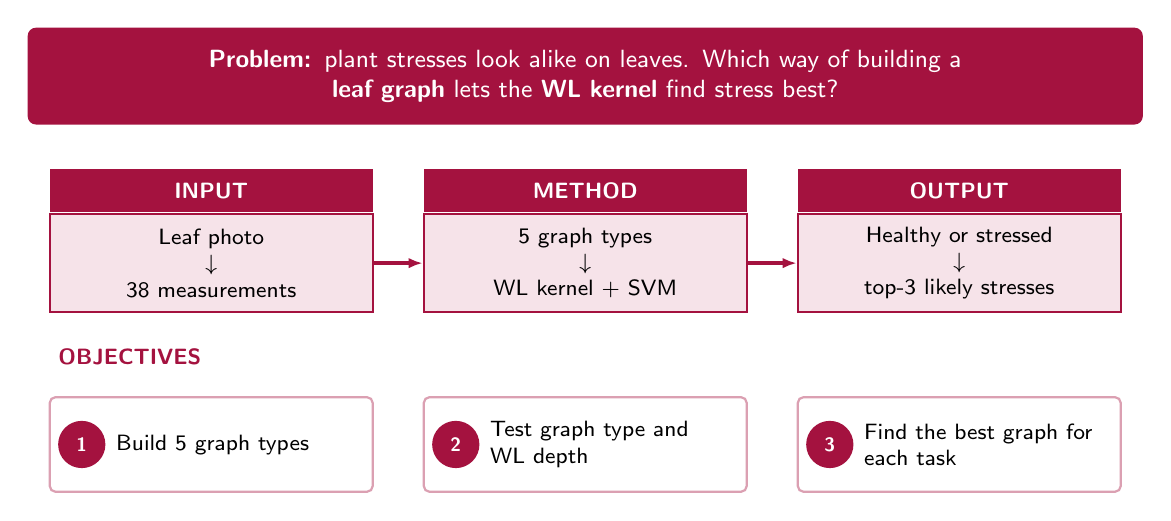
\begin{tikzpicture}[
        head/.style={rectangle, fill=amritaMaroon, text=white, font=\footnotesize\bfseries,
                     minimum width=4.1cm, minimum height=0.55cm, inner sep=2pt},
        body/.style={rectangle, draw=amritaMaroon, thick, fill=maroonSoft, font=\footnotesize,
                     text width=3.8cm, minimum width=4.1cm, minimum height=1.25cm, align=center, inner sep=4pt},
        goal/.style={rectangle, draw=amritaMaroon!40, thick, fill=white, rounded corners=2pt, font=\footnotesize,
                     text width=3.3cm, minimum width=4.1cm, minimum height=1.05cm, align=flush left, inner sep=4pt,
                     text depth=0pt, xshift=0cm},
        num/.style={circle, fill=amritaMaroon, text=white, font=\scriptsize\bfseries, minimum size=0.6cm, inner sep=0pt}
    ]
        % --- problem statement banner ---
        \node[rectangle, fill=amritaMaroon, text=white, rounded corners=3pt, text width=13.6cm,
              align=center, inner sep=8pt, font=\small] (q) at (0,0)
              {\textbf{Problem:} plant stresses look alike on leaves. Which way of building a\\
               \textbf{leaf graph} lets the \textbf{WL kernel} find stress best?};

        % --- input -> method -> output cards ---
        \node[head, below=0.55cm of q.south, xshift=-4.75cm, anchor=north] (h1) {INPUT};
        \node[body, below=0pt of h1] (b1) {Leaf photo\\$\downarrow$\\38 measurements};
        \node[head, below=0.55cm of q.south, anchor=north] (h2) {METHOD};
        \node[body, below=0pt of h2] (b2) {5 graph types\\$\downarrow$\\WL kernel + SVM};
        \node[head, below=0.55cm of q.south, xshift=4.75cm, anchor=north] (h3) {OUTPUT};
        \node[body, below=0pt of h3] (b3) {Healthy or stressed\\$\downarrow$\\top-3 likely stresses};
        \draw[arr, line width=1.2pt] (b1.east) -- (b2.west);
        \draw[arr, line width=1.2pt] (b2.east) -- (b3.west);

        % --- objectives ---
        \node[font=\footnotesize\bfseries, text=amritaMaroon, anchor=west] (ot) at ($(b1.south west)+(0,-0.55)$) {OBJECTIVES};
        \foreach \i/\txt in {1/{Build 5 graph types},
                             2/{Test graph type and WL depth},
                             3/{Find the best graph for each task}} {
            \node[goal, anchor=north, text width=0pt, minimum width=4.1cm, minimum height=1.2cm] (g\i) at ($(b\i.south)+(0,-1.05)$) {};
            \node[num] at ($(g\i.west)+(0.42,0)$) {\i};
            \node[font=\footnotesize, text width=3.0cm, align=flush left, anchor=west, inner sep=0pt]
                 at ($(g\i.west)+(0.85,0)$) {\txt};
        }
    \end{tikzpicture}
\end{frame}

\begin{frame}{1. Research Motivation}
    \begin{columns}[c]
        \column{0.56\textwidth}
        \small
        \begin{itemize}
            \setlength{\itemsep}{0.2cm}
            \item Many plant stresses look alike.
            \item Stress shows as a \textbf{mix} of signs -- e.g.\ yellow edges + normal shape.
            \item Normal models look at each measurement \textbf{alone}.
            \item A graph can show how measurements are \textbf{linked}.
        \end{itemize}

        \column{0.40\textwidth}
        \centering
        \traitgraph{0.85}

        {\scriptsize\itshape A leaf as a graph of measurements.}
    \end{columns}
    \vspace{0.35cm}
    \begin{center}
    
\begin{tikzpicture}
        \node[keybox, text width=0.85\textwidth] {\small \textbf{Gap:} a leaf is not a graph by itself. Nobody has tested how best to build one.};
    \end{tikzpicture}
    \end{center}
\end{frame}

\begin{frame}{What is the WL Graph Kernel?}
    \begin{columns}[c]
        \column{0.54\textwidth}
        \small
        The Weisfeiler--Lehman (WL) kernel \cite{shervashidze2011weisfeiler} measures how \textbf{similar two graphs} are.
        \vspace{0.25cm}

        \begin{itemize}
            \setlength{\itemsep}{0.15cm}
            \item Every node starts with a label.
            \item Each round, a node adds its neighbours' labels to its own.
            \item Graphs that share many labels are similar.
        \end{itemize}
        \vspace{0.2cm}
        {\scriptsize Used for molecules, proteins and program code \cite{borgwardt2005protein, li2016detecting}.}

        \column{0.46\textwidth}
        \centering
        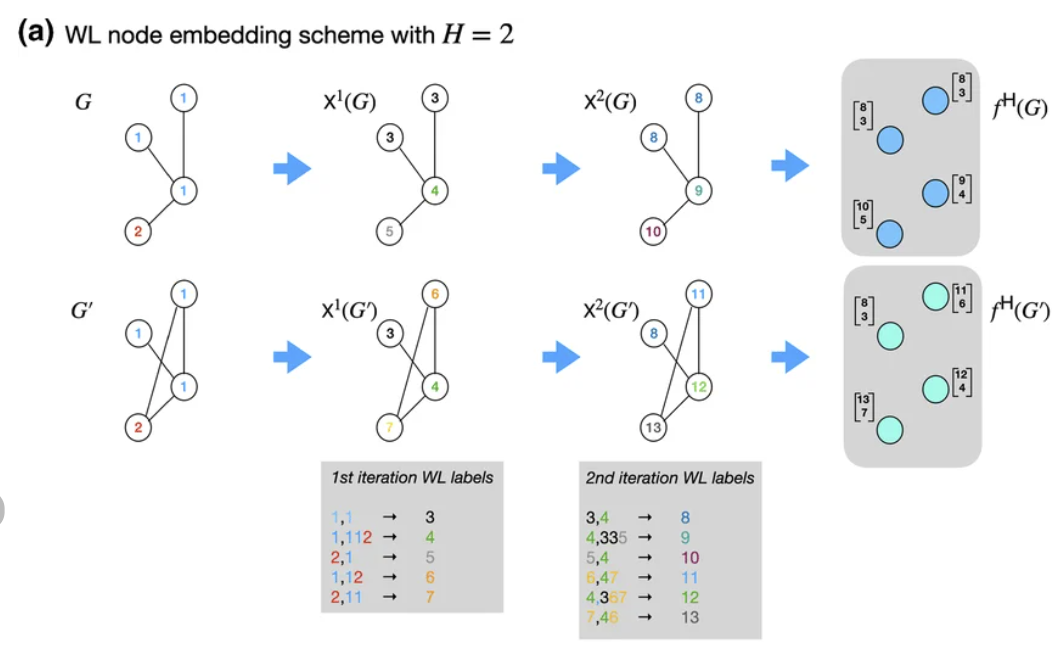
\includegraphics[width=\linewidth, height=0.85\textheight, keepaspectratio]{wl_demo.png}
    \end{columns}
\end{frame}

\begin{frame}{2. Proposed Methodology \& Overall Workflow}
    \centering
    \vspace{0.3cm}
    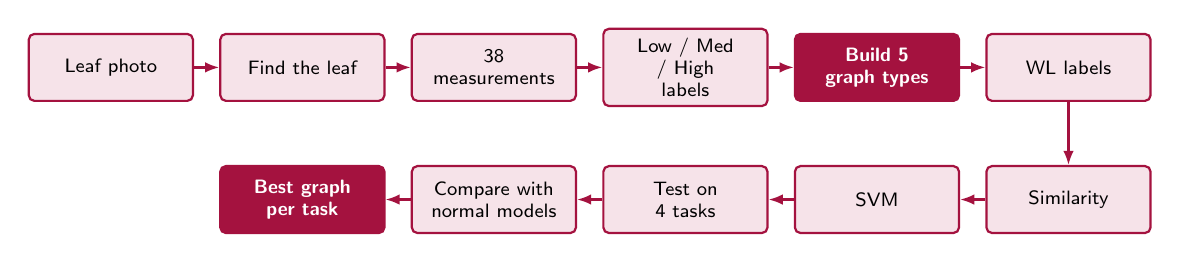
\begin{tikzpicture}[node distance=0.32cm]
        \node[flow] (a1) {Leaf photo};
        \node[flow, right=of a1] (a2) {Find the leaf};
        \node[flow, right=of a2] (a3) {38\\measurements};
        \node[flow, right=of a3] (a4) {Low / Med / High\\labels};
        \node[flowdark, right=of a4] (a5) {Build 5\\graph types};
        \node[flow, right=of a5] (a6) {WL labels};
        \node[flow, below=0.8cm of a6] (b1) {Similarity};
        \node[flow, left=of b1] (b2) {SVM};
        \node[flow, left=of b2] (b3) {Test on\\4 tasks};
        \node[flow, left=of b3] (b4) {Compare with\\normal models};
        \node[flowdark, left=of b4] (b5) {Best graph\\per task};
        \draw[arr] (a1) -- (a2); \draw[arr] (a2) -- (a3); \draw[arr] (a3) -- (a4);
        \draw[arr] (a4) -- (a5); \draw[arr] (a5) -- (a6); \draw[arr] (a6) -- (b1);
        \draw[arr] (b1) -- (b2); \draw[arr] (b2) -- (b3); \draw[arr] (b3) -- (b4);
        \draw[arr] (b4) -- (b5);
    \end{tikzpicture}
    \vspace{0.6cm}

    \small Leaf $\rightarrow$ graph $\rightarrow$ WL similarity $\rightarrow$ SVM $\rightarrow$ which graph works best?
\end{frame}

\begin{frame}{3. Methodological Components \& Formulation}
    \begin{columns}[T]
        \column{0.48\textwidth}
        \begin{block}{Parts}
            \small
            \begin{itemize}
                \item 38 measurements per leaf
                \item 5 graph types
                \item WL kernel + SVM
            \end{itemize}
        \end{block}
        \begin{block}{Data}
            \small
            \begin{itemize}
                \item OLID-I \cite{orka2023olid}: 8 crops, 4,387 leaves
                \item 5-fold cross-validation \cite{kohavi1995study}
            \end{itemize}
        \end{block}

        \column{0.48\textwidth}
        \begin{block}{Similarity of two leaves}
            \[ K(G,G') = \frac{\langle \phi(G), \phi(G') \rangle}{\|\phi(G)\|\,\|\phi(G')\|} \]
            \scriptsize $\phi(G)$ = how often each WL label appears. $K$ goes from 0 (different) to 1 (same).
        \end{block}
        \begin{block}{Score}
            \small Macro-F1: every class counts equally.
        \end{block}
    \end{columns}
\end{frame}

% =========================================================================
% SECTION 2: IMPLEMENTATION DETAILS
% =========================================================================
\section{Implementation Details}

\begin{frame}{Dataset: OLID Leaf Images}
    \begin{columns}[c]
        \column{0.50\textwidth}
        \small
        \begin{itemize}
            \setlength{\itemsep}{0.2cm}
            \item \textbf{OLID-I} \cite{orka2023olid}: 4,749 leaf photos
            \item 8 crops, 20 conditions
            \item Healthy, nutrient deficiency, pests, disease
        \end{itemize}

        \column{0.44\textwidth}
        \centering
        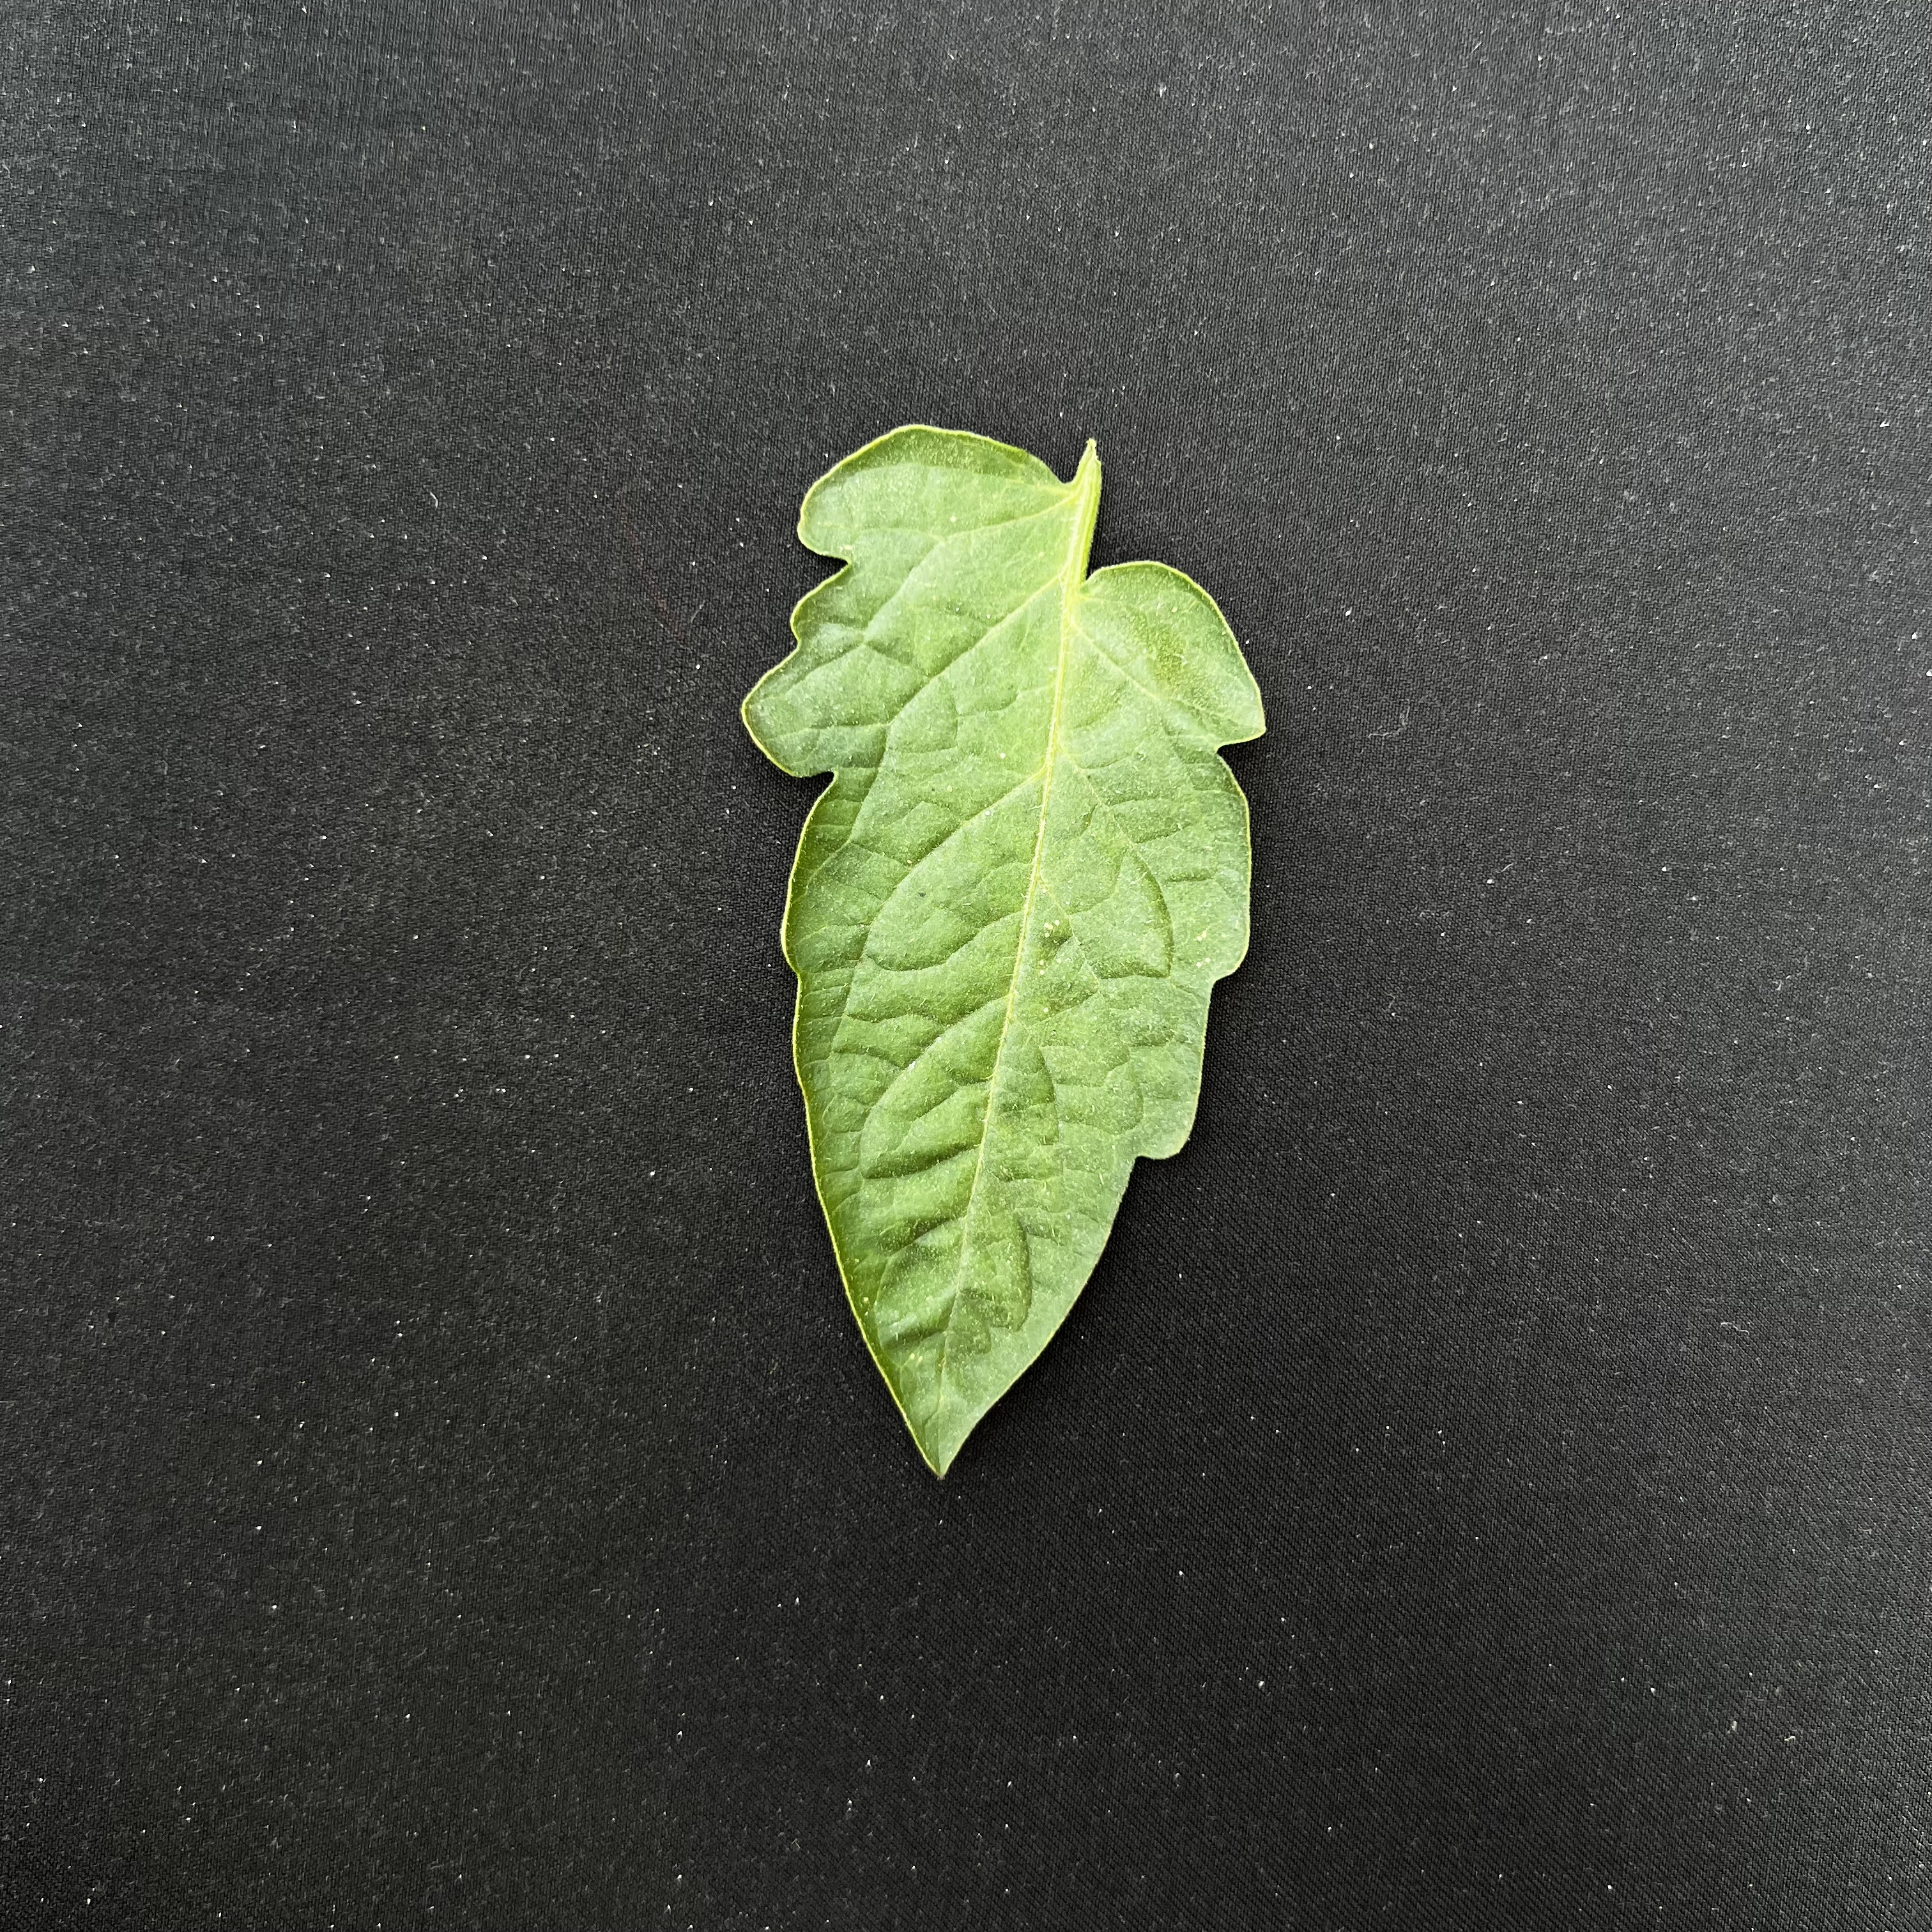
\includegraphics[width=0.85\linewidth, height=0.65\textheight, keepaspectratio]{leaf_sample.JPG}\\
        {\scriptsize\itshape A sample leaf photo}
    \end{columns}
\end{frame}

\begin{frame}{Finding the Leaf}
    \begin{columns}[c]
        \column{0.48\textwidth}
        \small
        \begin{itemize}
            \setlength{\itemsep}{0.2cm}
            \item Green-colour index + automatic threshold \cite{woebbecke1995color, otsu1979threshold}.
            \item Keep the leaf if it covers 1--98\% of the photo.
        \end{itemize}
        \vspace{0.3cm}
        \begin{center}
        \begin{tabular}{@{}lr@{}}
            \toprule
            Kept & \textbf{4,387 (92\%)} \\
            Removed & 362 \\
            \bottomrule
        \end{tabular}
        \end{center}

        \column{0.48\textwidth}
        \centering
        \begin{tikzpicture}
            \node[inner sep=0] (raw) {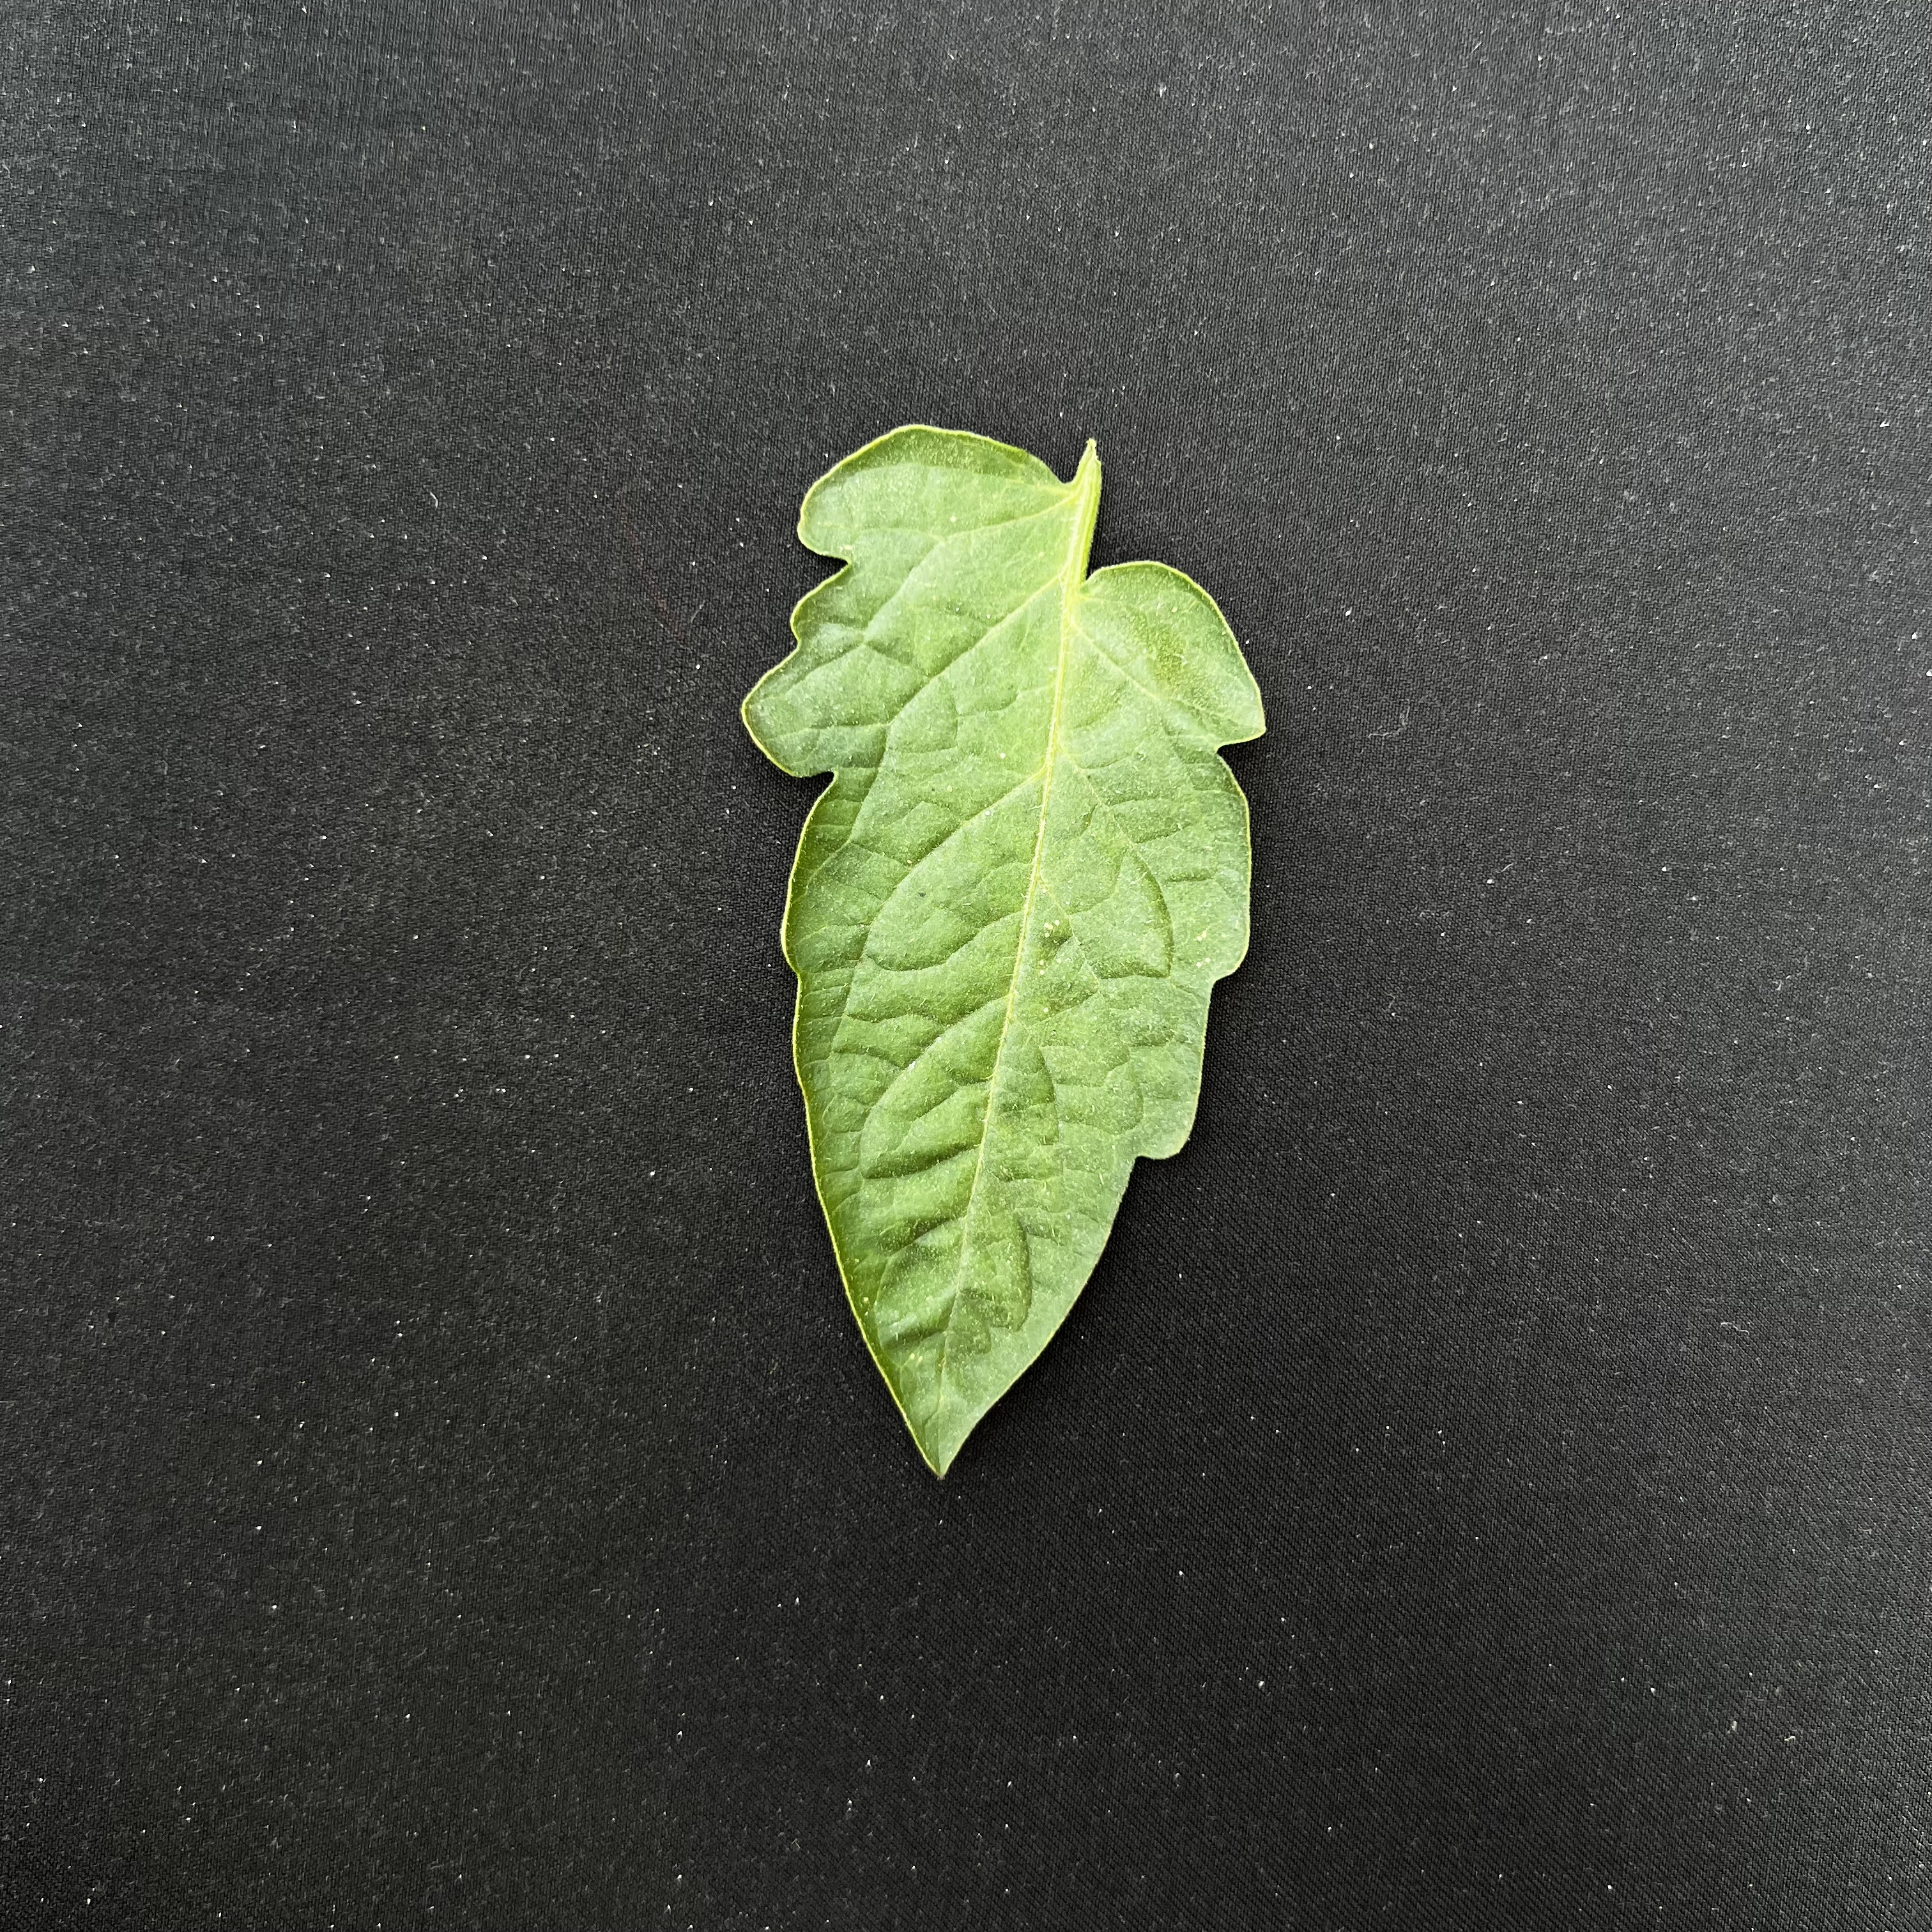
\includegraphics[height=3.0cm]{leaf_sample.JPG}};
            \node[inner sep=0, right=0.8cm of raw] (mask) {
\includegraphics[height=3.0cm]{segmentation_example.png}};
            \draw[arr] (raw) -- (mask);
            \node[below=0.1cm of raw, font=\scriptsize] {Photo};
            \node[below=0.1cm of mask, font=\scriptsize] {Leaf found};
        \end{tikzpicture}
    \end{columns}
\end{frame}

\begin{frame}{38 Measurements per Leaf}
    \centering
    \small
    \renewcommand{\arraystretch}{1.4}
    \begin{tabular}{@{}l c l@{}}
        \toprule
        \textbf{Group} & \textbf{Count} & \textbf{Examples} \\
        \midrule
        Shape & 10 & area, perimeter, roundness \\
        Colour & 20 & mean red / green / hue, yellow ratio \\
        Texture \cite{haralick1973textural} & 4 & contrast, smoothness \\
        Centre vs edge & 4 & yellow in the centre, yellow at the edge \\
        \bottomrule
    \end{tabular}
    \vspace{0.5cm}

    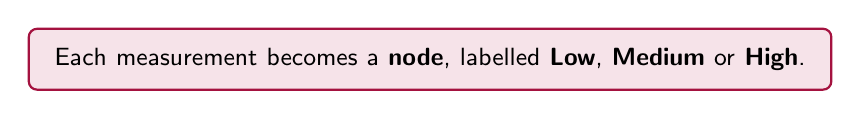
\begin{tikzpicture}
        \node[keybox, text width=0.8\textwidth] {\small Each measurement becomes a \textbf{node}, labelled \textbf{Low}, \textbf{Medium} or \textbf{High}.};
    \end{tikzpicture}
\end{frame}

\begin{frame}{The Five Graph Types}
    \centering
    \small
    \renewcommand{\arraystretch}{1.45}
    \begin{tabular}{@{}l l@{}}
        \toprule
        \textbf{Graph} & \textbf{Links measurements that\ldots} \\
        \midrule
        Correlation & rise and fall together \cite{pearson1895notes} \\
        $k$NN & are most similar (3 each) \cite{cover1967nearest} \\
        Feature-Family & are the same type (shape, colour, \ldots) \\
        Spatial & describe the leaf centre and edge \\
        Hybrid & are linked in Correlation, Family or Spatial \\
        \bottomrule
    \end{tabular}
    \vspace{0.4cm}

    {\footnotesize Same 38 nodes in every graph -- only the links change.}
\end{frame}

\begin{frame}{What the Five Graphs Look Like}
    \centering
    \begin{tabular}{ccc}
        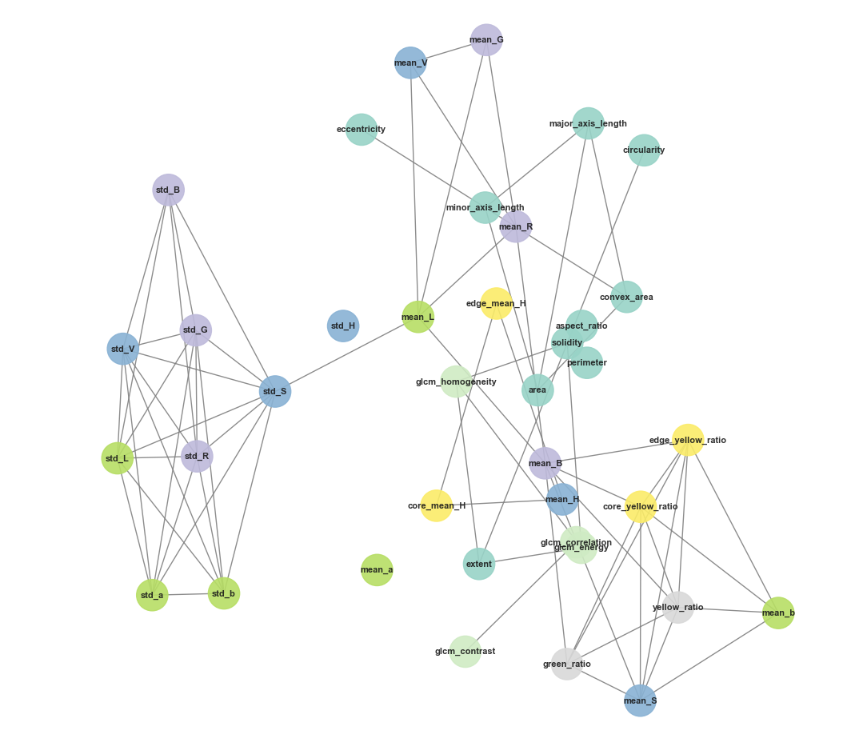
\includegraphics[height=0.33\textheight, width=0.30\textwidth, keepaspectratio]{correlation_graph.png} &
        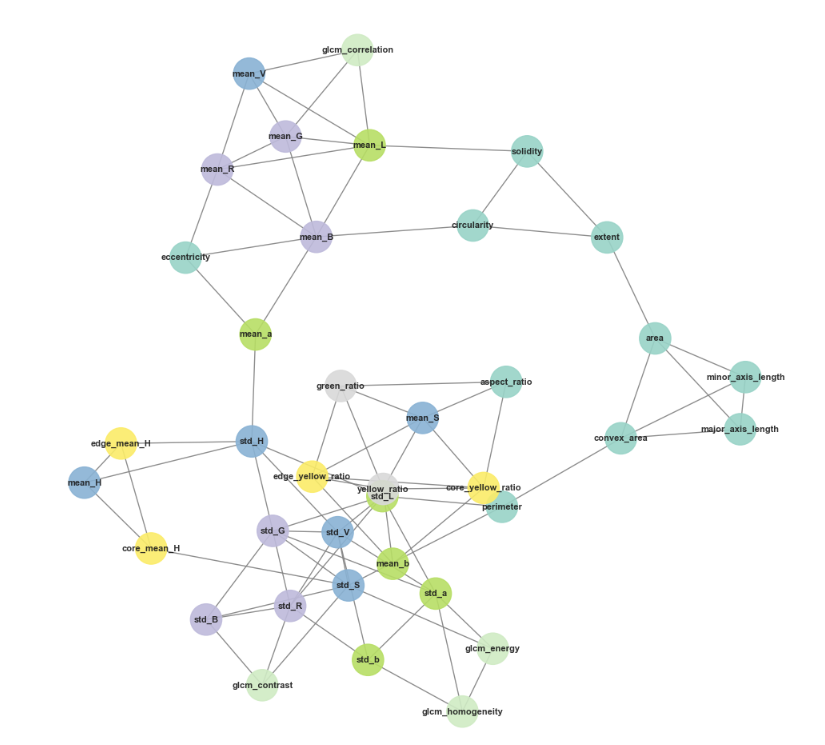
\includegraphics[height=0.33\textheight, width=0.30\textwidth, keepaspectratio]{knn_Graph.png} &
        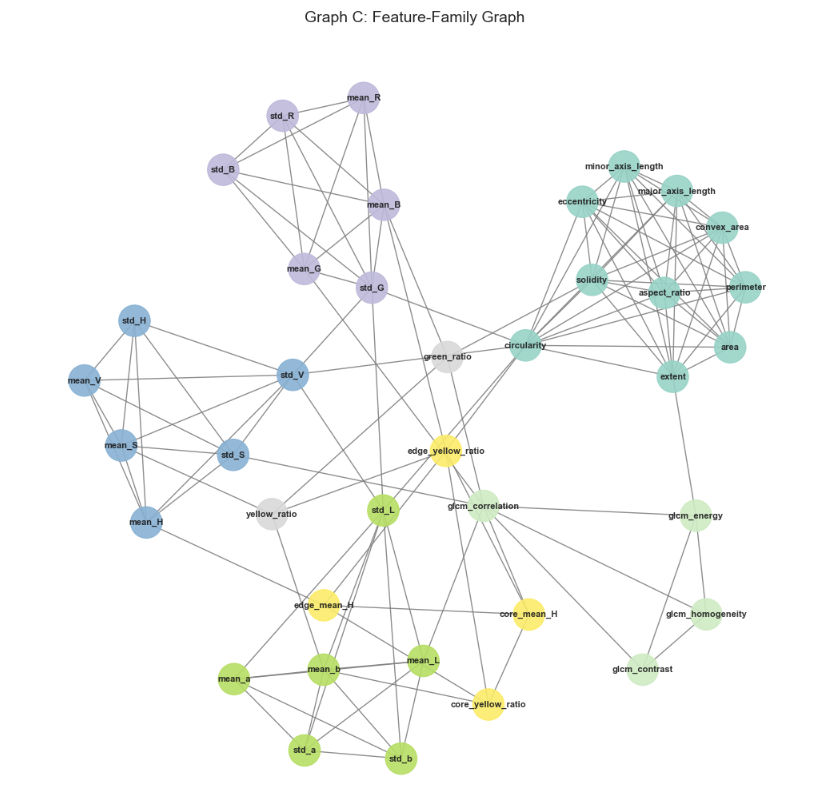
\includegraphics[height=0.33\textheight, width=0.30\textwidth, keepaspectratio]{feature_family.png} \\
        {\scriptsize Correlation} & {\scriptsize $k$NN} & {\scriptsize Feature-Family} \\[0.15cm]
        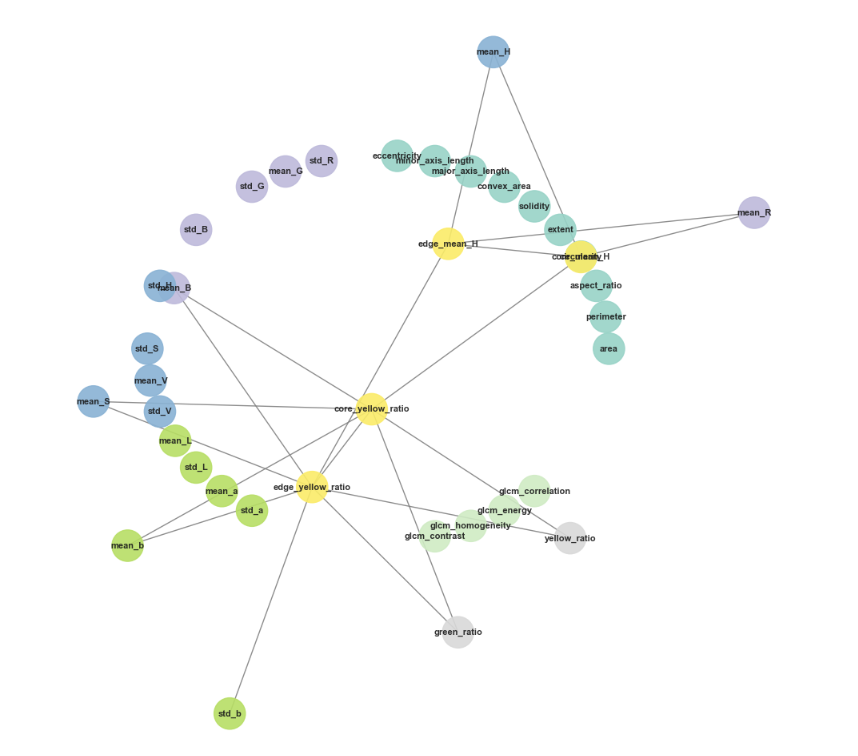
\includegraphics[height=0.33\textheight, width=0.30\textwidth, keepaspectratio]{spatial_graph.png} &
        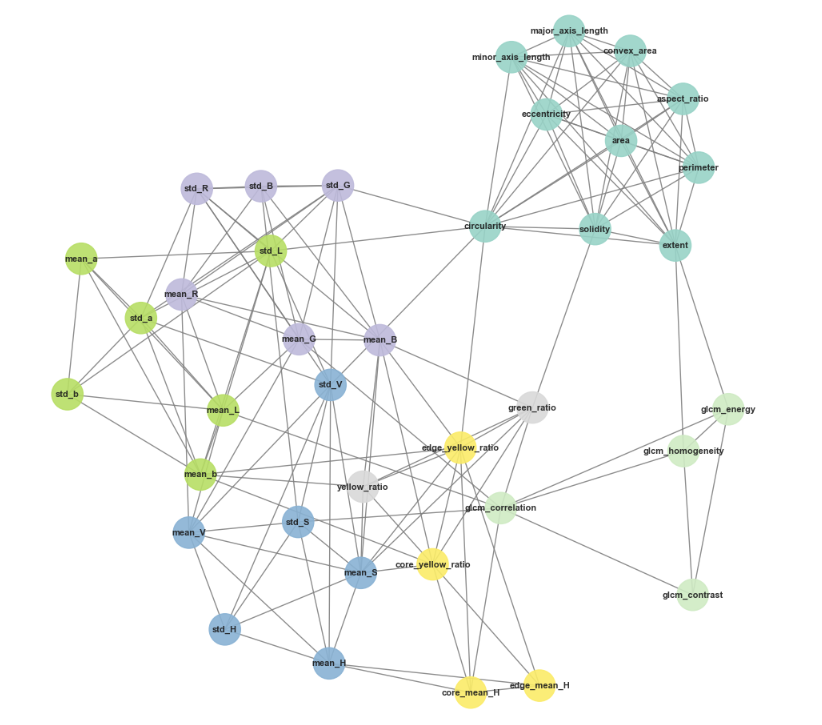
\includegraphics[height=0.33\textheight, width=0.30\textwidth, keepaspectratio]{hybrid_graph.png} &
        \begin{minipage}[b][0.30\textheight][c]{0.27\textwidth}
            \raggedright\footnotesize Fewest links: Spatial (19)\\[0.1cm] Most links: Hybrid (147)
        \end{minipage} \\
        {\scriptsize Spatial} & {\scriptsize Hybrid} & \\
    \end{tabular}
\end{frame}

\begin{frame}{4. Core Module Implementation Details}
    \begin{columns}[c]
        \column{0.50\textwidth}
        \small
        \begin{itemize}
            \setlength{\itemsep}{0.2cm}
            \item WL runs for depth $h = 0$ to $3$.
            \item At $h = 0$ links are ignored -- our ``no graph'' baseline.
            \item Labels are learned from training leaves only.
            \item SVM \cite{cortes1995support} classifies using the similarity.
        \end{itemize}

        \column{0.44\textwidth}
        \centering
        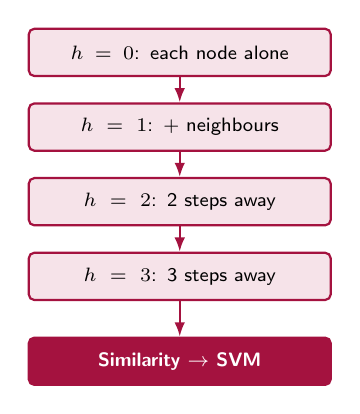
\begin{tikzpicture}[node distance=0.32cm]
            \tikzset{vs/.style={flow, text width=3.6cm, minimum height=0.6cm}}
            \node[vs] (s0) {$h=0$: each node alone};
            \node[vs, below=of s0] (s1) {$h=1$: + neighbours};
            \node[vs, below=of s1] (s2) {$h=2$: 2 steps away};
            \node[vs, below=of s2] (s3) {$h=3$: 3 steps away};
            \node[vs, below=0.45cm of s3, fill=amritaMaroon, text=white, font=\scriptsize\bfseries] (v) {Similarity $\rightarrow$ SVM};
            \draw[arr] (s0) -- (s1); \draw[arr] (s1) -- (s2); \draw[arr] (s2) -- (s3); \draw[arr] (s3) -- (v);
        \end{tikzpicture}
    \end{columns}
\end{frame}

% =========================================================================
% SECTION 3: VERIFICATION & DEMONSTRATION (results: 2 pages)
% =========================================================================
\section{Verification \& Demonstration}

\begin{frame}{5. Preliminary Verification \& Quantitative Results}
    \framesubtitle{Healthy vs stressed, all crops: macro-F1 in \% (average of 5 folds)}
    \centering
    \small
    \renewcommand{\arraystretch}{1.1}
    \begin{tabular}{@{}l c@{}}
        \toprule
        \textbf{Model} & \textbf{Healthy vs stressed} \\
        \midrule
        Always answers ``stressed'' (reference) & 45.6 \\
        Random Forest \cite{breiman2001random} (default) & 65.2 \\
        RBF SVM (default) & 66.4 \\
        \midrule
        WL, no graph ($h=0$) & 60.1 \\
        WL + Spatial & 62.2 \\
        WL + Correlation & 62.2 \\
        WL + $k$NN & 67.4 \\
        WL + Feature-Family & 69.1 \\
        \textbf{WL + Hybrid} & \textbf{69.7} \\
        \bottomrule
    \end{tabular}
    \vspace{0.3cm}

    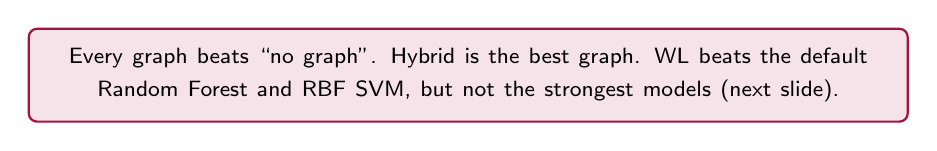
\begin{tikzpicture}
        \node[keybox, text width=0.88\textwidth] {\footnotesize Every graph beats ``no graph''. Hybrid is the best graph. WL beats the default Random Forest and RBF SVM, but not the strongest models (next slide).};
    \end{tikzpicture}
\end{frame}

\begin{frame}{5. Fair Benchmark: Where WL Stands}
    \framesubtitle{Full pipeline (find the crop, then that crop's stress model): macro-F1 in \%}
    \begin{columns}[T]
        \column{0.50\textwidth}
        \small
        \renewcommand{\arraystretch}{1.08}
        \begin{tabular}{@{}l c@{}}
            \toprule
            \textbf{Model} & \textbf{Macro-F1} \\
            \midrule
            CNN EfficientNet-B0 (frozen) & 73.9 \\
            Extra Trees (tuned) & 72.9 \\
            Gradient Boosting (tuned) & 72.1 \\
            \textbf{WL + SVM} (best setting) & \textbf{70.6} \\
            WL + SVM (tuned the same way) & 68.3 \\
            Random Forest (default) & 68.2 \\
            Always answers ``stressed'' & 45.6 \\
            \bottomrule
        \end{tabular}

        {\scriptsize All models: same 5 folds; tuned = settings chosen inside each training fold only.}

        \column{0.46\textwidth}
        \begin{block}{Robustness (photo changed 7 ways)}
            \scriptsize Drop in F1: CNN $\approx 0$; \textbf{WL $-5.3$}, the smallest of all feature-based models; boosting $-7.5$ to $-12.6$; Random Forest $-17.6$.
        \end{block}
        \begin{block}{Why not accuracy?}
            \scriptsize 84\% of leaves are stressed: always answering ``stressed'' already gives 83.8\% accuracy, so we report macro-F1.
        \end{block}
        \begin{block}{Speed (photo $\rightarrow$ answer)}
            \scriptsize CNN $\approx$ 0.14\,s; every 38-measurement model $\approx$ 1.1\,s (full-size segmentation), so the CNN is $\approx 8\times$ faster.
        \end{block}
        \begin{block}{Explainability}
            \scriptsize Only WL explains a decision with named leaf measurements and how they are linked.
        \end{block}
    \end{columns}
    \vspace{0.15cm}
    \centering
    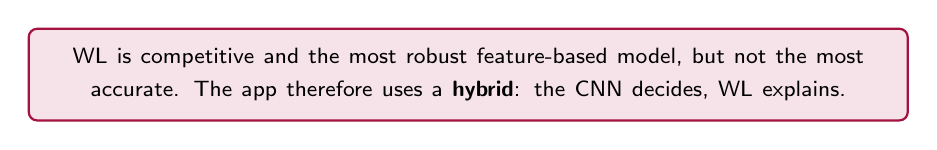
\begin{tikzpicture}
        \node[keybox, text width=0.88\textwidth] {\footnotesize WL is competitive and the most robust feature-based model, but not the most accurate. The app therefore uses a \textbf{hybrid}: the CNN decides, WL explains.};
    \end{tikzpicture}
\end{frame}

\begin{frame}{5. Where WL Stands Out: A Second Opinion Farmers Can Trust}
    \framesubtitle{CNN decides, WL checks and explains (all 4,387 leaves, held-out folds)}
    \begin{columns}[T]
        \column{0.52\textwidth}
        \small
        \renewcommand{\arraystretch}{1.12}
        \begin{tabular}{@{}l c c@{}}
            \toprule
            & \textbf{Leaves} & \textbf{CNN correct} \\
            \midrule
            \textcolor{green!50!black}{\textbf{$\bullet$ CNN and WL agree}} & 83\% & \textbf{91\%} \\
            \textcolor{orange!90!black}{\textbf{$\bullet$ CNN and WL disagree}} & 17\% & 56\% \\
            \midrule
            CNN alone (all leaves) & 100\% & 85\% \\
            \bottomrule
        \end{tabular}

        \vspace{0.25cm}
        {\footnotesize Disagreement flags only \textbf{17\%} of leaves but contains \textbf{51\%} of all CNN mistakes;
        the CNN's own confidence catches 44\% at the same rate.}

        \column{0.44\textwidth}
        \begin{block}{For the farmer}
            \scriptsize \textcolor{green!50!black}{\textbf{Green}}: both agree $\rightarrow$ act on it.\\
            \textcolor{orange!90!black}{\textbf{Amber}}: they disagree $\rightarrow$ check the leaf or ask an expert.
        \end{block}
        \begin{block}{Explains why}
            \scriptsize e.g.\ ``greenness lower and edge yellowness higher than healthy tomato leaves'', in leaf terms, not pixels.
        \end{block}
        \begin{block}{Stays stable in the field}
            \scriptsize Least quality loss of all measurement-based models when light, blur or camera change.
        \end{block}
    \end{columns}
    \vspace{0.1cm}
    \centering
    {\scriptsize Other measurement-based models give a similar warning, but none of them explains itself in leaf terms or is as stable.}
\end{frame}

\begin{frame}{5. Limitation: The Exact Condition (57 Classes)}
    \begin{columns}[T]
        \column{0.50\textwidth}
        \small
        \begin{itemize}
            \setlength{\itemsep}{0.2cm}
            \item OLID-I has \textbf{57} crop $\times$ condition classes.
            \item Our 38 measurements are \textbf{averages over the whole leaf}.
            \item Many conditions differ only in \textbf{small local marks} (mite dots, miner trails, spots); averages wash them out.
            \item Best model on these measurements: \textbf{57.0\%} macro-F1; WL: 42.3\%.
        \end{itemize}
        \vspace{0.1cm}
        {\scriptsize So naming the exact condition in one step is a stated limitation, not our main task.}

        \column{0.46\textwidth}
        \centering
        {\small \textbf{Instead: a top-3 shortlist per crop}}\\[0.1cm]
        \scriptsize
        \renewcommand{\arraystretch}{1.05}
        \begin{tabular}{@{}l c c@{}}
            \toprule
            \textbf{Crop} & \textbf{1st} & \textbf{In top 3} \\
            \midrule
            Cucumber & 57\% & \textbf{98\%} \\
            Tomato & 69\% & \textbf{96\%} \\
            Snake gourd & 64\% & \textbf{94\%} \\
            Ridge gourd & 55\% & \textbf{91\%} \\
            Ash gourd & 59\% & \textbf{90\%} \\
            Bottle gourd & 53\% & 86\% \\
            Eggplant & 49\% & 84\% \\
            Bitter gourd & 48\% & 83\% \\
            \bottomrule
        \end{tabular}

        {\scriptsize WL condition model, 5-fold CV}
    \end{columns}
    \vspace{0.15cm}
    \centering
    
\begin{tikzpicture}
        \node[keybox, text width=0.88\textwidth] {\footnotesize We answer ``healthy or stressed'', and give the exact condition as a shortlist for an expert to confirm.};
    \end{tikzpicture}
\end{frame}

\begin{frame}{6. Experimental Visualizations \& Prototype Demonstration}
    \begin{columns}[T]
        \column{0.49\textwidth}
        \centering
        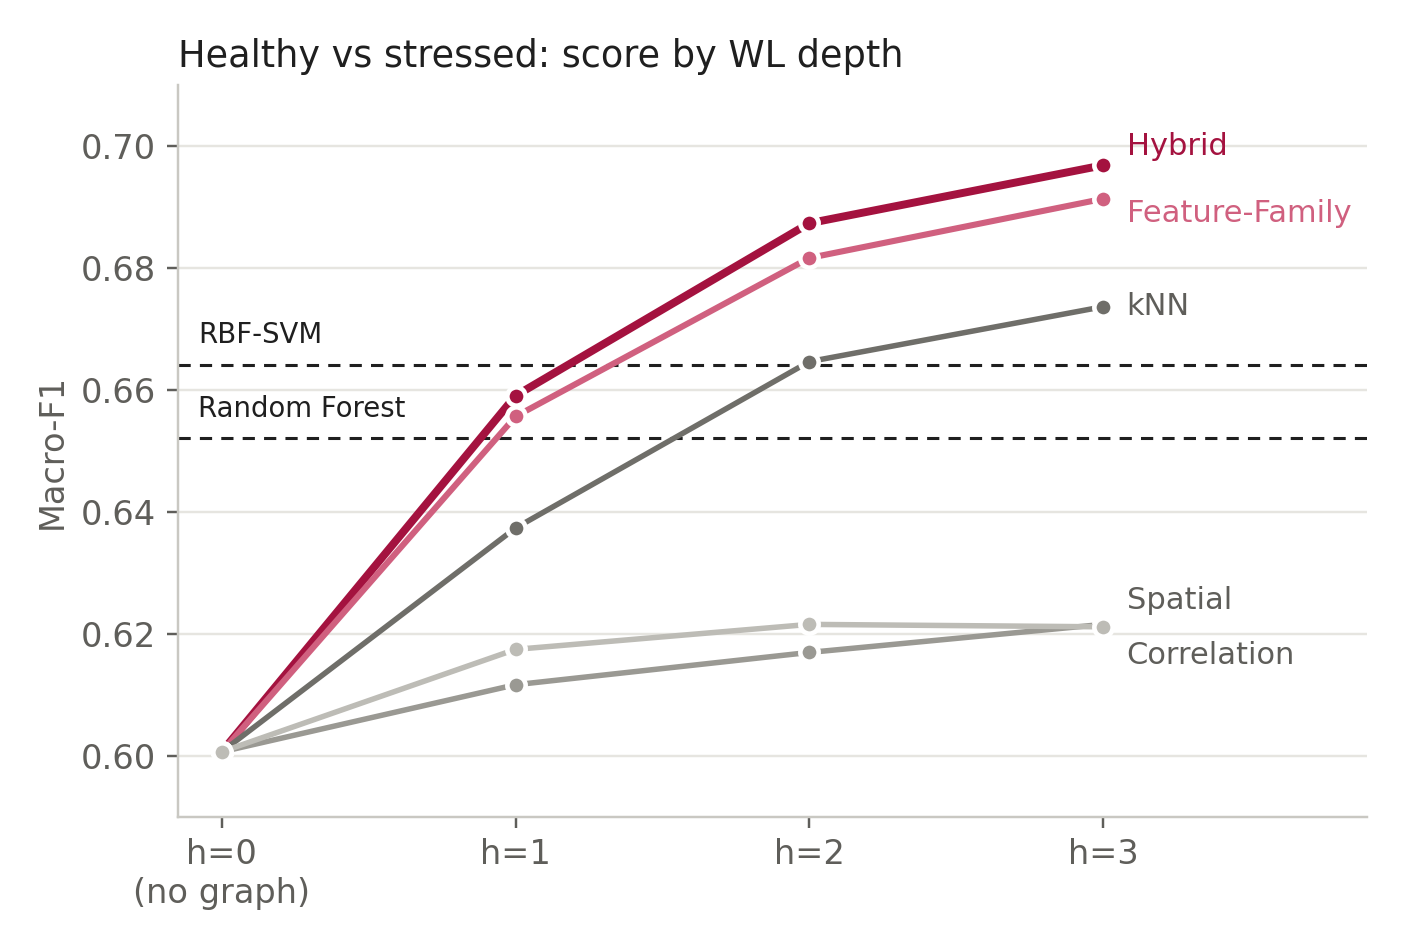
\includegraphics[width=\linewidth, height=0.6\textheight, keepaspectratio]{wl_height_sweep.png}\\
        {\footnotesize Deeper WL helps.}

        \column{0.49\textwidth}
        \centering
        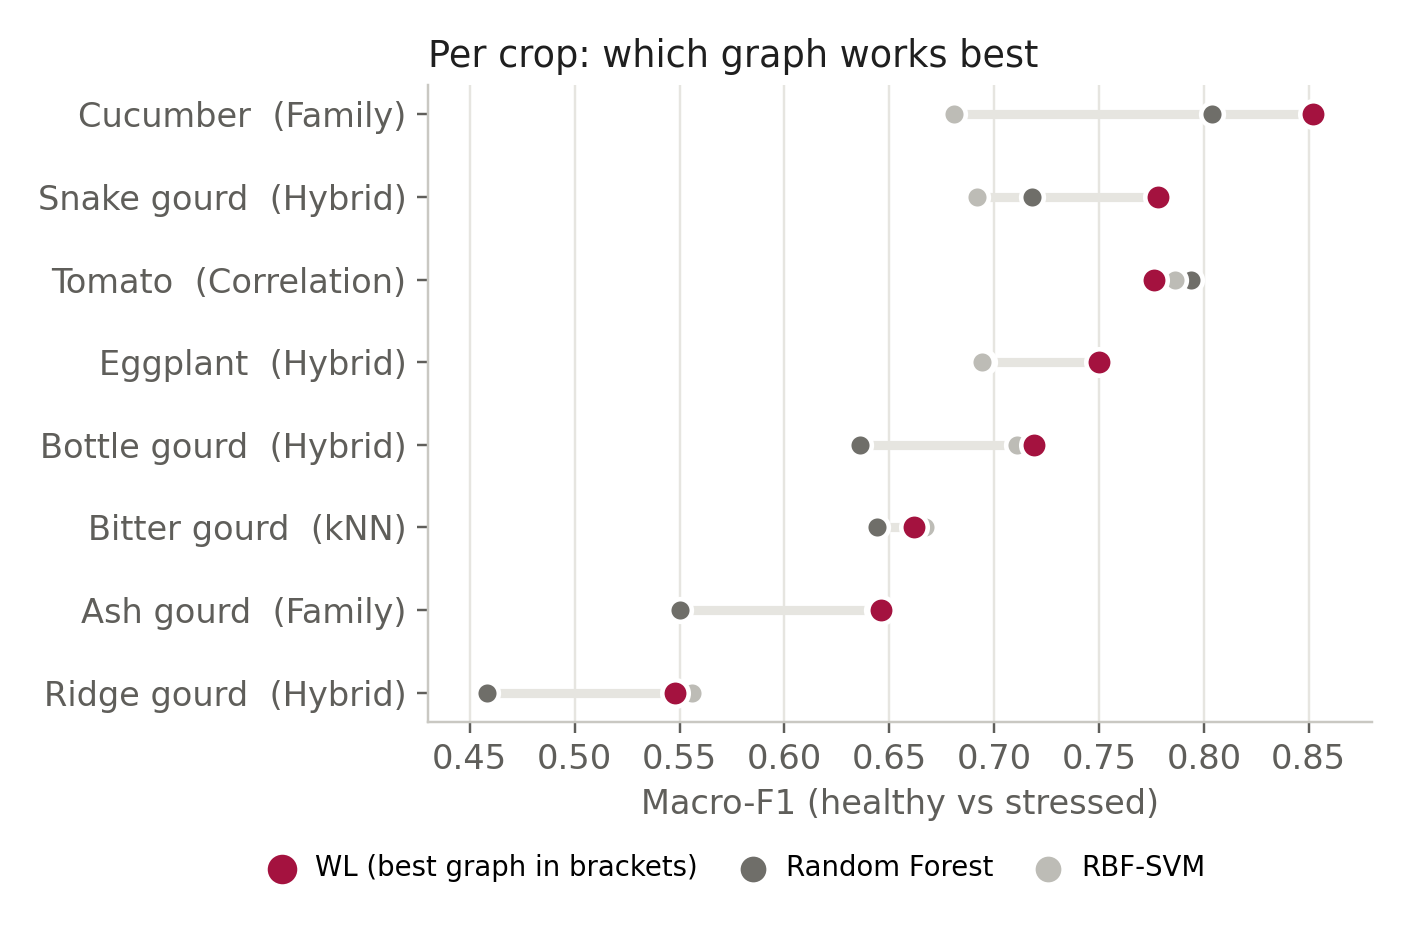
\includegraphics[width=\linewidth, height=0.6\textheight, keepaspectratio]{per_crop_l2.png}\\
        {\footnotesize The best graph changes by crop.}
    \end{columns}
    \vspace{0.2cm}
    \centering
    {\footnotesize \textbf{Live demo:} PlantCare AI -- a CNN makes the call, WL explains it step by step and gives a second opinion.}
\end{frame}

% =========================================================================
% SECTION 4: TECHNICAL KNOWLEDGE
% =========================================================================
\section{Technical Knowledge}

\begin{frame}{7. Technical Justification, Design Trade-offs \& Insights}
    \begin{columns}[T]
        \column{0.48\textwidth}
        \begin{block}{Why WL?}
            \small Its labels are easy to read -- each is a mix of measurements.
        \end{block}
        \begin{block}{Trade-off}
            \small Deeper WL finds more detail, but makes many more labels.
        \end{block}

        \column{0.48\textwidth}
        \begin{block}{Edge Cases}
            \small Bad leaf photos are removed; unseen labels are skipped.
        \end{block}
        \begin{block}{Next Steps}
            \small Local spot measurements for the exact condition; a fine-tuned CNN as a stronger reference.
        \end{block}
    \end{columns}
\end{frame}

\begin{frame}{Conclusion}
    \small
    \begin{enumerate}
        \setlength{\itemsep}{0.35cm}
        \item \textbf{Graphs help:} every graph beats ``no graph''.
        \item \textbf{Hybrid} is the best graph overall.
        \item \textbf{No single winner:} the best graph depends on the crop.
        \item \textbf{Fair benchmark:} WL is competitive and the most robust feature-based model; tuned trees and a CNN score higher.
        \item \textbf{Limitation:} the exact condition (57 classes) needs local measurements; we give a top-3 shortlist instead.
    \end{enumerate}
    \vspace{0.3cm}
    \begin{center}
    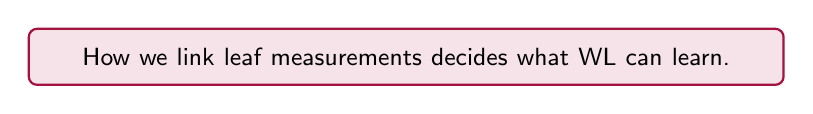
\begin{tikzpicture}
        \node[keybox, text width=0.75\textwidth] {\small How we link leaf measurements decides what WL can learn.};
    \end{tikzpicture}
    \end{center}
\end{frame}

% =========================================================================
% REFERENCES & THANK YOU
% =========================================================================
\section{References}
\begin{frame}[allowframebreaks]{References}
    \tiny
    \bibliographystyle{ieeetr}
    \bibliography{ref}
\end{frame}

\begin{frame}
    \centering
    {\Huge \textbf{\textcolor{amritaMaroon}{Thank You}}} \\[0.4cm]
    {\large \textbf{Questions \& Viva Voce}}
\end{frame}

\end{document}
